% !TeX root = main.tex


\begin{savequote}[70mm]
,,Mapy mają dwie zasadnicze cechy: nie są terytorium, które opisują, ale, jeśli
są zrobione poprawnie, mają podobną do nich strukturę, co powoduje o~ich
przydatności.''
\qauthor{Alfred Korzybski}
\end{savequote}


\chapter{System nawigacji}
\label{chap:mapa}

\section{Struktura systemu nawigacji}

Wybór struktury programowej ROS pociągnął za sobą w~sposób naturalny kolejne
wybory związane ze strukturą systemu nawigacji robota. Zgodnie z~filozofią
twórców tego oprogramowania, podsystem nawigacji dla robota mobilnego podzielony
jest na kilka modułów, których wzajemna współpraca i~zależności pokazane są na
rysunku~\ref{fig:diag_move_base}. Część z~nich jest dostarczana razem z~systemem
ROS i~wykorzystywana bez zmian w~kodzie (of the shelf), niektóre mogą być
swobodnie wymieniane pod warunkiem, że spełniają wymogi odpowiednich interfejsów
(razem z~systemem dostarczone są pewne implementacje, z~których można
skorzystać), wymagane jest też dostarczenie kilku modułów zależnych od samego
robota, na którym całość jest uruchamiana.

\begin{figure}[h!]
\centering
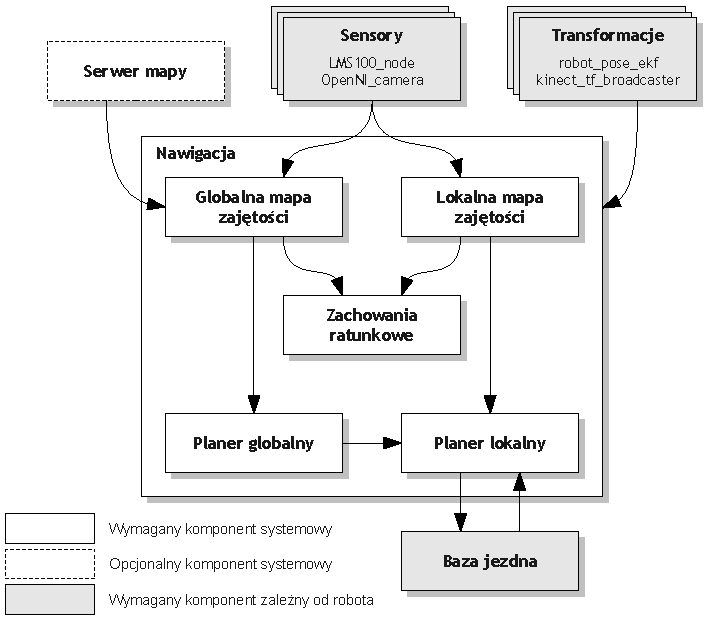
\includegraphics{../img/diag_move_base}
\caption{Struktura systemu nawigacji robota}
\label{fig:diag_move_base}
\end{figure}

Modułami, które są dostarczone i~niezmienne są mapy przeszkód (konkretnie
moduły agregujące dane z~sensorów i~tworzące na ich podstawie mapy zajętości).
Modułami wymiennymi są planery trasy (zarówno lokalny jak i~globalny) oraz
zachowania awaryjne mające na celu wyprowadzenie robota z~trudnych sytuacji
(np. otoczenie przeszkodami). Dodatkowo wymagane jest dostarczenie przynajmniej
modułów sensorycznych, modułów określających lokalizację robota w~pewnym,
globalnym układzie współrzędnych (może to być układ związany z~punktem startowym
robota) oraz oczywiście głównego sterownika robota. Ogólnie cały system można
podzielić na trzy główne części, odpowiedzialne za wykrywanie przeszkód 
i~tworzenie lokalnych map zajętości (kosztu), lokalizację robota oraz planowanie
trasy (globalne i~lokalne).

\section{Tworzenie map przeszkód}

Podczas poruszania się robota w~środowisku o~nie w~pełni znanej strukturze
kluczowe jest wykrywanie aktualnej konfiguracji przeszkód. W~środowiskach
statycznych wystarczy samo ich zaznaczanie na mapie, w~przypadku otoczenia
dynamicznie się zmieniającego równie ważne jest wykrywanie momentów, w~których
przeszkody znikają (czyszczenie przeszkód na mapie jest trudniejsze niż ich
oznaczanie). Cały proces wykrywania i~oznaczania przeszkód można podzielić na
cztery etapy:

\begin{itemize}
  \item agregacja danych z~sensorów,
  \item filtrowanie danych,
  \item oznaczanie przeszkód w~pewnej, wybranej strukturze danych,
  \item tworzenie dwuwymiarowej mapy kosztu.
\end{itemize}

\subsection{Agregacja danych z~czujników}

Pierwszym etapem jest zebranie danych z~sensorów. W~przypadku robota Elektron
istnieją dwa źródła danych o~przeszkodach -- skaner laserowy SICK oraz sensor
Kinect. Biorąc pod uwagę wielkość otrzymywanych danych (w~przypadku lasera
kilkaset punktów, w~przypadku sensora Kinect kilka tysięcy na każdy pomiar) oraz
stosunkowo niewielką prędkość poruszania się robota, do wykrywania przeszkód
nie są wykorzystywane wszystkie odczyty, a~jedynie pięć na sekundę w~przypadku
lasera oraz dwa na sekundę w~przypadku Kinecta.

Po zebraniu pomiarów muszą one jeszcze zostać przetransformowane do wspólnego
układu współrzędnych, w~tym przypadku do układu związanego z~bazą robota 
(w~przypadku sensora Kinect należy także wziąć pod uwagę jego pochylenie względem
bazy). Za publikację wszystkich niezbędnych transformacji  odpowiedzialne są
komponenty \comp{kinect\_tf\_broadcaster} oraz \comp{laser\_tf}.

\subsection{Filtrowanie danych}

Dane odebrane z~sensorów podlegają dalszemu procesowi filtracji, który ma na
celu usunięcie odczytów w~jakikolwiek sposób zafałszowanych. Odczyty ze skanera
laserowego są obarczone takimi błędami w~sposób niewielki, dlatego w~tym
przypadku filtracja się nie odbywa. Inaczej przedstawia się kwestia odczytów 
z~Kinecta -- pojawiające się w~nich pojedyncze, przypadkowe punkty mogą powodować
pojawianie się na mapie przeszkód uniemożliwiających ruch robota. Z tego powodu
stosowana jest filtracja danych ze względu na otoczenie punktów -- pojedyncze
odczyty, odstające od reszty pomiarów (posiadające w~otoczeniu zbyt mało
sąsiadów) są odrzucane.

\subsection{Mapa wokselowa}

Wszystkie punkty, które przejdą przez proces filtracji, są przekazywane do
modułu tworzącego mapę zajętości. Wewnętrznie przechowuje on reprezentację
otoczenia w~postaci mapy wokselowej (trójwymiarowa siatka prostopadłościanów).
Zmieniając wielkość oczek siatki możemy wybierać pomiędzy dokładnością pokrycia
otoczenia (im większe oczka, tym przeszkody będą zajmowały więcej miejsca, nawet małe
przeszkody będą reprezentowane przez całe zajęte oczka siatki) a~szybkością
działania i~obciążeniem systemu (małe oczka wymagają dużo większego nakładu
obliczeniowego). Implementacja dostępna w~systemie ROS ze względów
optymalizacyjnych zakłada maksymalnie 16 poziomów siatki w~pionie, nie jest to
jednak ograniczenie w~sposób szczególny wpływające na jej użyteczność. Dzięki
przyjętemu sposobowi reprezentacji (każda kolumna w~mapie reprezentowana przy
pomocy jednej liczby całkowitej) można było natomiast zastosować wydajne
algorytmy śledzenia promieni (wykorzystywane przy czyszczeniu przeszkód z~mapy).

Największym ograniczeniem tej struktury danych jest założenie, że robot porusza
się po płaskim terenie, na którym nie występują spadki (np. schody w~dół), przez
co przeszkody o~,,ujemnej wysokości'' nie są w~żaden sposób wykrywane. Niestety,
moduł odpowiedzialny za tworzenie map otoczenia nie jest przystosowany do
łatwego dostarczania własnych implementacji wewnętrznych struktur danych 
i~algorytmów (tak jak np. planery trasy). Istniały dwie możliwości
rozwiązania tego problemu: stworzenie kopii dużej części systemu i~wprowadzanie
w~niej własnych zmian, bądź napisanie modułu pośredniczącego pomiędzy sensorem 
a~algorytmami oznaczania przeszkód, która to metoda została wybrana.

\begin{figure}[htb!]
\centering
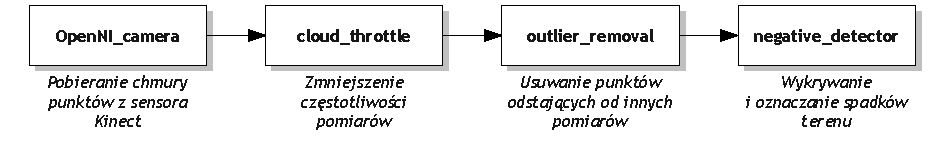
\includegraphics{../img/filtering}
\caption{Potok przetwarzania chmury punktów z~sensora Kinect}
\label{fig:filtering}
\end{figure}

\subsubsection{Wykrywanie spadków terenu}

Przed przekazaniem danych z~sensora Kinect do dalszych algorytmów tworzenia map
przeszkód są one przetwarzane przez zestaw filtrów. Pierwszy z~nich usuwa punkty
odstające w~pewien sposób od reszty pomiaru, a~więc takie, które mogą sugerować
szum pomiarowy. Punkty te są wykrywane przez zliczanie sąsiadów w~ich otoczeniu
o~określonej wielkości, a~jeśli tych sąsiadów będzie mniej niż dwóch, punkt taki
jest odrzucany z~dalszych obliczeń.

\begin{figure}[htb!]
\centering
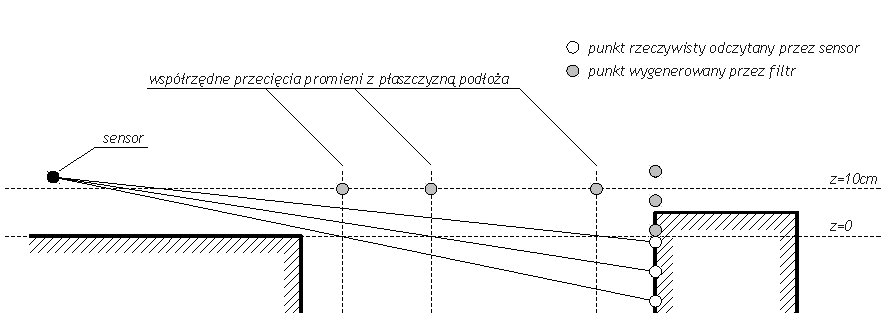
\includegraphics{../../Common/img/depresion}
\caption{Wykrywanie spadków terenu}
\label{fig:depresion}
\end{figure}

Kluczowym filtrem jest jednak wykrywanie spadków terenu. Zostało ono zrealizowane
w~sposób koncepcyjnie dość prosty, dający jednak bardzo dobre rezultaty. Dla punktów
o~współrzędnej $z>0$ wykonywane
jest proste przepisanie bez żadnych zmian, natomiast punkty poniżej progu są przekazywane
do dalszej obróbki. W~pierwszym kroku są one odbijane względem płaszczyzny $z=0$
(a więc punkt o~współrzędnych $(x, y, z)$ zamieniany jest na punkt o~współrzędnych
$(x, y, -z)$). Jako, że zazwyczaj wykrywane są przeszkody dopiero w~pewnej
odległości od spadku terenu (patrz rysunek~\ref{fig:depresion}), konieczne jest
znalezienie właściwego miejsca spadku. W~tym celu wyznaczane jest równanie prostej
łączącej aktualnie badany punkt ze środkiem sensora, a~z niego wyliczane są współrzędne
$x$ oraz $y$ miejsca przecięcia tej prostej z~płaszczyzną $z=0$. Do chmury dodawane
są dodatkowe punkty o~współrzędnych $x$ i~$y$ wyliczonych wcześniej oraz współrzędnej
$z=0.1$ (symulowana jest przeszkoda znajdująca się 10cm ponad poziomem podłoża).
W ten sposób lokalny planer trasy jest niejako zmuszany do omijania spadków terenu.

\subsubsection{Czyszczenie przeszkód}

Pierwszym krokiem po dostarczeniu przetworzonej wstępnie chmury punktów do algorytmu
oznaczającego przeszkody jest oczyszczenie mapy z~przeszkód, które nie są już widoczne.
Dla każdego punktu z~danego pomiaru wykonywany jest ten sam algorytm. Pomiędzy
bieżącym punktem a~środkiem sensora z~którego pochodzi dany pomiar prowadzony jest
odcinek prostej, a~każda komórka mapy, przez który dany odcinek przechodzi jest
czyszczona z~przeszkód. Jako, że mapa jest dyskretna i~ma stosunkowo duże oczka,
do wyznaczania kolejnych komórek przez które przechodzi bieżący promień wykorzystany
został algorytm Bresenhama (rozszerzony na przypadek trójwymiarowy). Ogólnie czyszczenie
przeszkód z~mapy jest zadaniem dość czasochłonnym, widać też, że w~przyjętym algorytmie
do wyczyszczenia nieistniejących przeszkód konieczne jest istnienie innej przeszkody
tak, aby odpowiednie punkty pojawiły się w~chmurze z~pomiaru (jeśli nie będzie możliwości
poprowadzenia promienia przez dany punkt z~powodu braku odpowiednich pomiarów, to
przeszkoda taka nie zniknie z~mapy). Własność ta sprawia, że tworzenie lokalnych
map zajętości o~zbyt dużych rozmiarach może spowodować problemy (przypadkowe przeszkody
pojawiające się w~otwartym terenie daleko od robota mogą nigdy nie zostać wyczyszczone).

\subsubsection{Oznaczanie przeszkód}

Oznaczanie przeszkód wykonywane po oczyszczeniu poprzedniego stanu mapy jest zadaniem
dużo prostszym, zarówno koncepcyjnie jak i~obliczeniowo. Dla każdego punktu z~danego
pomiaru wyznaczana jest komórka, w~której dany punkt leży, a~następnie jest ona
oznaczana jako zajęta.

Kolejność wykonywanych działań, a~więc najpierw czyszczenie, a~dopiero potem
oznaczanie nowych przeszkód ma kluczowe znaczenie. Gdyby wykonywane było jednocześnie
dla każdego punktu i~czyszczenie, i~oznaczanie przeszkód, mogłoby dochodzić do
sytuacji, w~których dopiero co oznaczone w~mapie obiekty byłyby usuwane przez proces
czyszczenia wywoływany dla innych punktów z~danego pomiaru.


\subsection{Mapa zajętości}

Po zaznaczeniu wszystkich przeszkód w~mapie wokselowej, są one rzutowane na
dwuwymiarową mapę zajętości. Wszystkie kolumny, w~których są oznaczone zajęte
komórki są oznaczane jako zajęte, jeśli natomiast w~kolumnie są tylko komórki
puste bądź nieznane, to w~zależności od ilości nieznanych oznaczenie jest różne.
Jeśli więcej niż 4 komórki są nieznane, wtedy cała kolumna jest uznawana za
nieznaną, w~przeciwnym wypadku kolumna jest uznawana za pustą.

Po oznaczeniu przeszkód dokonywane jest ich powiększenie na określoną odległość
(nadmuchiwanie). Operacja ta ma na celu wygładzenie mapy kosztu i~spowodowanie,
że robot nie będzie preferował szerokie przejazdy (o ile będzie miał wybór). NA
rysunku~\ref{fig:inflation} przedstawiona jest ogólna metoda obliczania kosztu
dla komórki podczas tego procesu. Parametrem kontrolującym ten proces jest
promień ,,nadmuchiwania'', od którego zależy, jak dużą odległość od
przeszkód będzie zachowywał robot.

\begin{figure}[htb!]
\centering
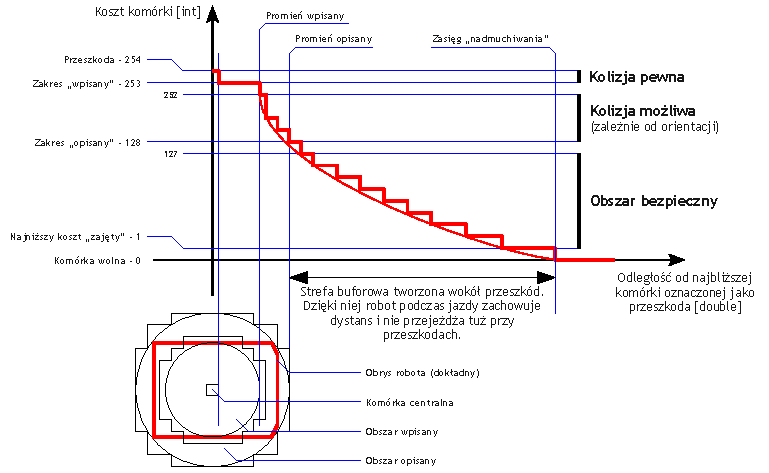
\includegraphics[width=15cm]{../../Common/img/ros/inflate.pdf}
\caption{Nadmuchiwanie przeszkód.}
\label{fig:inflation}
\end{figure}

Mapa zajętości ma stały rozmiar, a~jej środek związany jest ze środkiem bazy
jezdnej robota. W~środowiskach o~dynamicznie zmieniającej się konfiguracji
przeszkód przechowywanie globalnej mapy zajętości (innej niż statyczna mapa
otoczenia) często powoduje więcej problemów niż pożytku -- przeszkody widoczne
na niej w~dużej odległości od robota mogą faktycznie już zniknąć, a~pozostając
na mapie mogą zakłamywać globalne planowanie ścieżki. Dodatkowo wprowadzona jest
duża oszczędność pamięci, gdyż przechowywana mapa ma stały rozmiar, niezależnie
od przejechanego przez robota dystansu i~wielkości eksplorowanego środowiska.

\section{Lokalizacja robota}

Obliczanie względnej pozycji robota (a więc liczona na podstawie jego ruchu, względem
punktu początkowego) zostało opisane już wcześniej przy okazji opisu odometrii
oraz rozszerzonego filtru Kalmana. W~przypadku aplikacji, gdzie nie jest wykorzystywany
żaden system lokalizacji globalnej jest to jedyne źródło informacji o~położeniu,
użytkownik może dodatkowo wskazać na mapie położenie początkowe aby umożliwić pracę
globalnego planera trasy.

Możliwe jest także zastosowanie algorytmu globalnej lokalizacji -- jest to element
wymienny w~systemie nawigacji i~może być tam zastosowany dowolny gotowy bądź zaimplementowany
w~ramach badań algorytm. Jest to więc jeden z~elementów, które mogą być testowane
przy użyciu stworzonej platformy badawczej -- sama wymiana modułu lokalizacji jest
bardzo łatwa i~sprowadza się jedynie do uruchomienia własnego procesu z~algorytmem
w~miejsce istniejącego. W~szczególności jako algorytm lokalizacji globalnej może być
podany program wykorzystujący jedynie odometrię (tak jak zostało to opisane w~poprzednim
akapicie).

Do celów globalnego wyznaczania trasy oraz ewentualnej globalnej lokalizacji stworzona
została mapa kilku pomieszczeń, po których poruszał się robot. Jej tworzenie było
dwuetapowe -- najpierw przy pomocy algorytmu SLAM i~skanera laserowego zostały
stworzone mapy poszczególnych pomieszczeń (w~kilku częściach, ze względu na możliwości
obliczeniowe komputera sterującego). Mapy te zawierały oczywiście wszystkie bieżące
przeszkody i~ruchome elementy wyposażenia, takie jak stoły, krzesła czy pudła.
Na podstawie tych map stworzona została ręcznie w~programie typu CAD oczyszczona
mapa, zawierająca jedynie ściany pomieszczeń, duże meble (takie, których przestawienie
nie jest w~łatwy sposób możliwe, a~więc szafy pancerne i~ciężkie biurka warsztatowe)
oraz niedostępny dla robotów mobilnych podest z~manipulatorami. Wszystkie pozostałe
elementy (w~szczególności mniejsze stoły, krzesła czy kosze na śmieci) zostały z~tej
mapy usunięte.

W przygotowanych aplikacjach jako do nawigacji globalnej (względem dostarczonej
zgrubnej mapy środowiska) został wykorzystany algorytm AMCL (Adaptive Monte Carlo
Localization~\cite{fox2001kld}) wykorzystujący filtr cząsteczkowy do śledzenia
pozycji robota na znanej mapie. Pozycja jest wyznaczana na podstawie odczytów
ze skanera laserowego oraz z~układu odometrii robota. Ważne jest to, że pojawiające
się wokół robota przeszkody, które nie są umieszczone na mapie, nie wpływają znacząco
na jakość lokalizacji (dopóki robot przez dłuższy czas nie będzie nimi całkowicie
otoczony), oraz że algorytm szybko odnajduje właściwe położenie robota po jego
chwilowym zagubieniu. Algorytm bardzo dobrze radzi sobie z~lokalizowaniem robota nawet
posiadając jedynie zgrubną mapę otoczenia zawierającą kluczowe cechy otoczenia
(opisaną wcześniej).

\section{Planowanie trasy}

\subsection{Ścieżka globalna}

Po wskazaniu punktu docelowego uruchamiany jest globalny planer trasy. Element ten
jest wymienny i~może być wykorzystana implementacja dowolnego algorytmu (spełniająca
warunki narzucone przez interfejs systemu), tak więc jest to kolejny element, na którym
mogą być przeprowadzane eksperymenty używając stworzonej platformy. W~aplikacjach
testowych został wykorzystany algorytm Dijkstry wyszukiwania ścieżki w~grafie tworzonym
na podstawie mapy globalnej. Początkowo uwzględniana jest jedynie sama mapa, bez
dodatkowej informacji o~przeszkodach, a~w momencie, kiedy robot nie zdoła wykonać
zadanego planu, algorytm uruchamiany jest ponownie uwzględniając już przeszkody
z~dynamicznie tworzonej mapy zajętości wokół robota (które w~szczególności mogą
przesłaniać niektóre przejazdy, np. zamknięte drzwi).

Planer globalny wprowadza dodatkowe założenia o~kształcie robota -- przyjmuje, że
jest on okrągły i~do obliczeń wykorzystuje okrąg opisany na faktycznym obrysie robota.
Wynikają z~tego drobne problemy tego podejścia, mianowicie może się okazać, że nie
zostanie wyznaczona żadna ścieżka mimo, iż w~przy pewnej konfiguracji robot zmieściłby
się pomiędzy przeszkodami (np. przejeżdżając ,,na styk'' pomiędzy nimi). Sytuacja
taka nie wystąpiła jednak w~czasie eksperymentów, a~kształt robota Elektron jest
na tyle zwarty, że dla celów globalnego planowania trasy może być przybliżony okręgiem.

\subsection{Ścieżka lokalna}

Po wyznaczeniu planu globalnego jego fragmenty są przesyłane do lokalnego planera
trasy działającego z~wykorzystaniem algorytmu okna dynamicznego (opisany 
w~rozdziale~\ref{chap:nawigacja}). Obliczenia wykorzystują lokalną mapę zajętości
tworzoną wokół robota (z nanoszonymi na nią na bieżąco przeszkodami) oraz
bieżące odczyty z~układu odometrii robota (aktualna prędkość).
Funkcja liczenia kosztu ruchu jest ustawiona tak,
aby najmniejszym kosztem obarczone były trajektorie kończące się blisko ścieżki globalnej,
natomiast odjeżdżanie od niej owocowało zwiększaniem kosztu. Dużym problemem okazało
się dobranie odpowiednich parametrów algorytmu (a więc ograniczeń na prędkości
oraz długości pojedynczego kroku czasowego symulacji). Przy zbyt długim kroku
algorytm często wybierał ruch obrotowy z~niewielką prędkością liniową, który skutkował
powrotem do punktu wyjścia (koszt takiego ruchu był minimalny, gdyż kończył się dokładnie
na wyznaczonej ścieżce). Po eksperymentach i~ustawieniu parametrów robot wykonywał
wyznaczone ścieżki z~dużą szybkością (ok. 15cm/s, a~więc 75\% maksymalnej prędkości
dozwolonej dla robota) sprawnie unikając pojawiających się przeszkód.
